\chapter{Results and discussion}
\lhead{Results and discussion}


\section{Limb's angle correction}
Since we already take into account $\theta_\text{ZENITH}$ shifted due to Earth's radial asymmetry, we should see the count distribution versus $\theta_\text{NADIR}$ with lesser standard deviation as Figure 4.1.

\begin{figure}[h!]
    \centering
      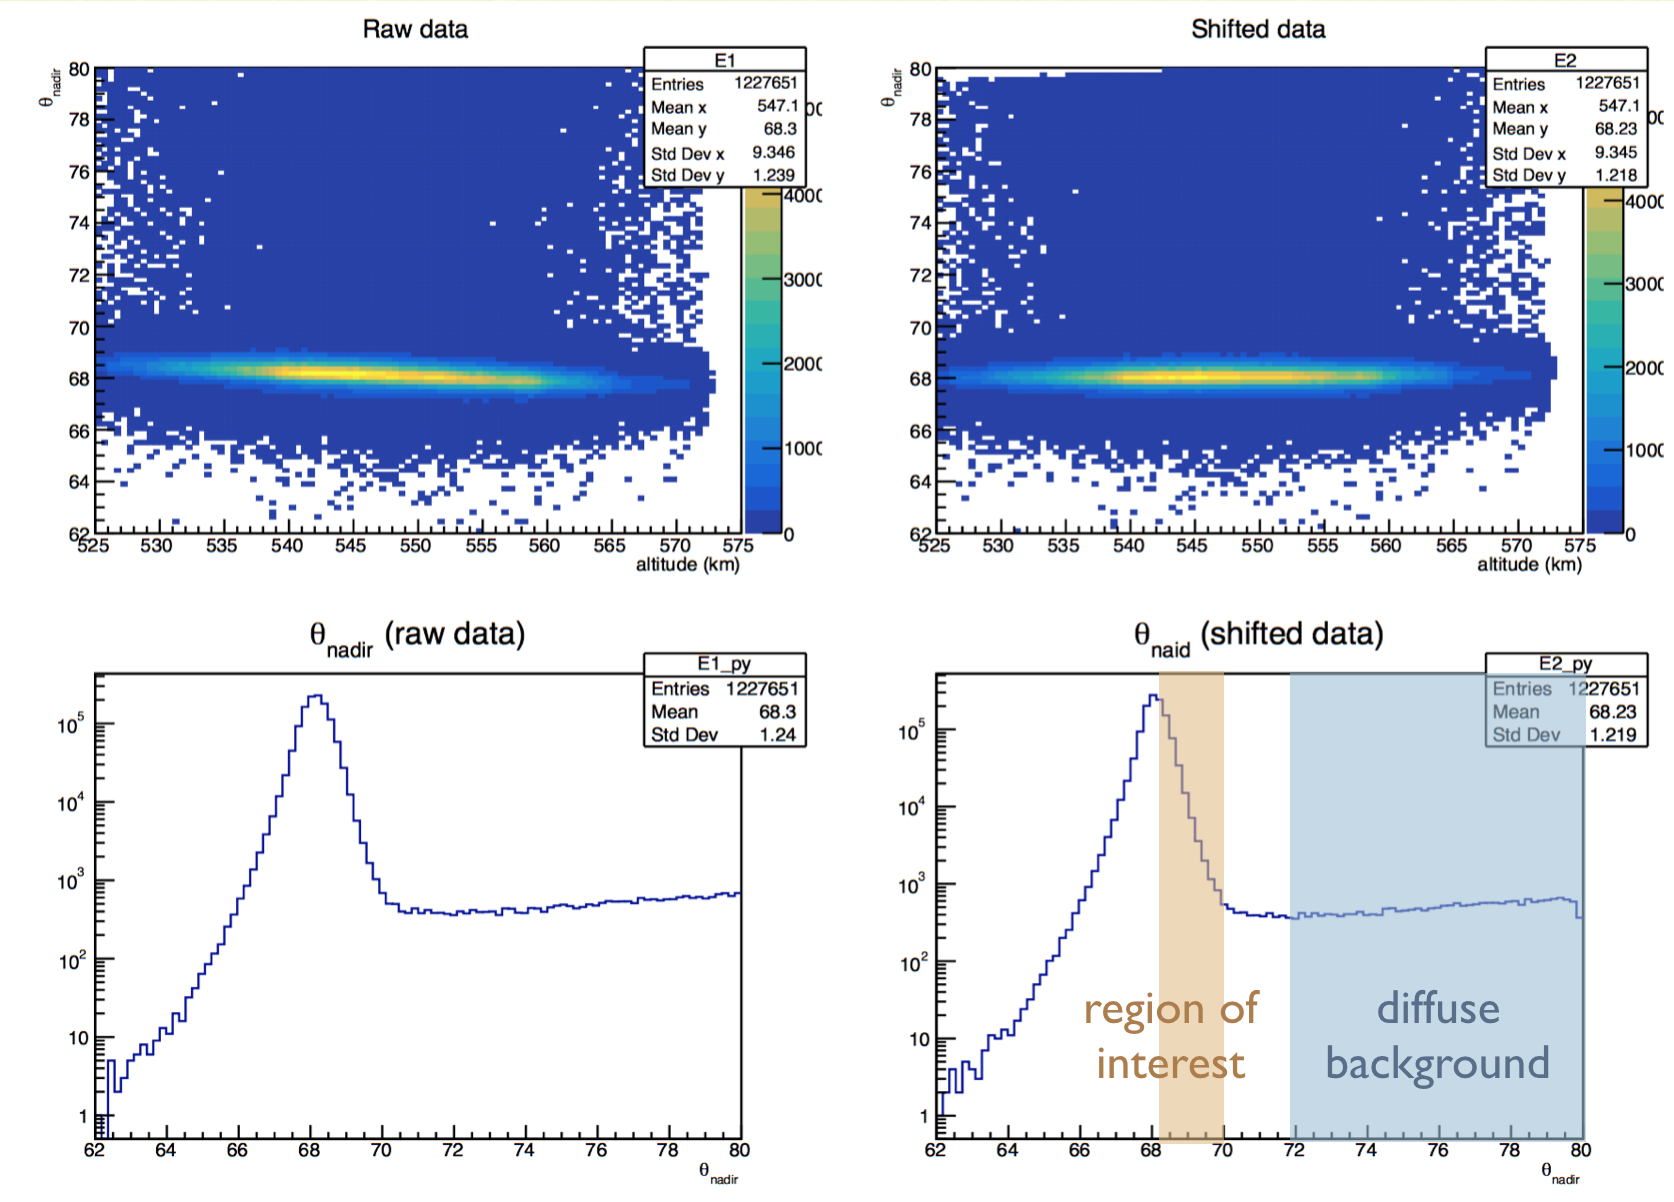
\includegraphics[width=\textwidth]{img/LATShifted}
      \caption{Distribution of nadir angle before and after altitude correction}
\end{figure}

%%%%%%%%%%%%%%%%%%%%%%%%%%%%%%%
%%%%%  gamma-ray spectrum   %%%
%%%%%%%%%%%%%%%%%%%%%%%%%%%%%%%
\section{$\gamma$-ray spectrum}
In this section, we provide an example of various map that we use in Earth's angular coordinate. Please note that we pick only 4 various energy bin to demenstrate by starting with Figure 4.2 for fill a raw event in the map. 
In order to get an exposure map, we have to dive deep to spacecraft log file to simulate field of view of LAT for count time in each grid on geologic's angular coordinate as well as regard effective area of LAT in different angle as shown in Figure 4.3. Intensity map of photon has a characteristics identification of west and north side like in Fig 4.4, it is obvious to see that west side has higher density than east side because geomagnetic cutoff rigidity when this effect dominated in a lower rigidity.
Finally, $\gamma$-ray spectrum as in Figure 4.5 could be computed from count map and exposure map with a calculation of Eq (3.1).
%%% show any map & flux
\begin{figure}[h!]
    \begin{tikzpicture}
    \node (0,0) {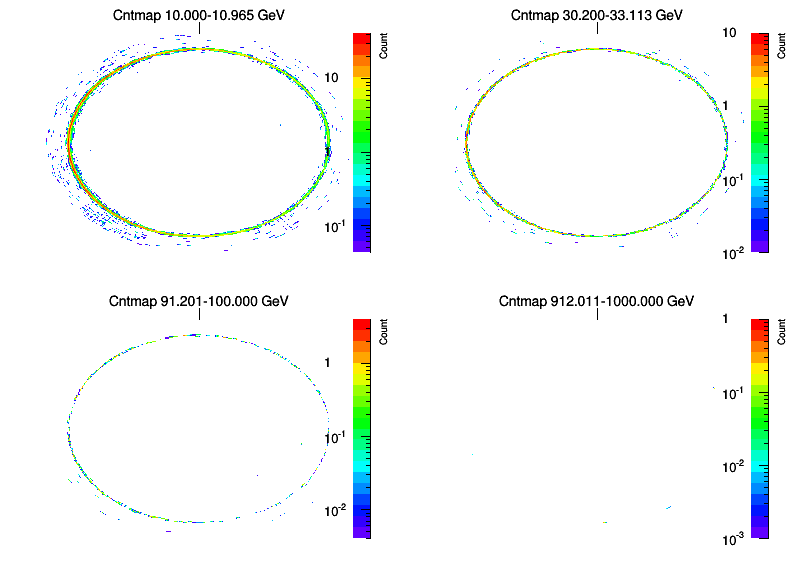
\includegraphics[width=\textwidth]{img/cntmapAfterCut}};
    \node [opacity=0.2] (0,0) {\rotatebox{45}{\scalebox{3.0}{\textcolor{red}{preliminary}}}};
    \end{tikzpicture}
    \caption{Count map}
\end{figure}


\begin{figure}[h!]
    \begin{tikzpicture}
    \node (0,0) {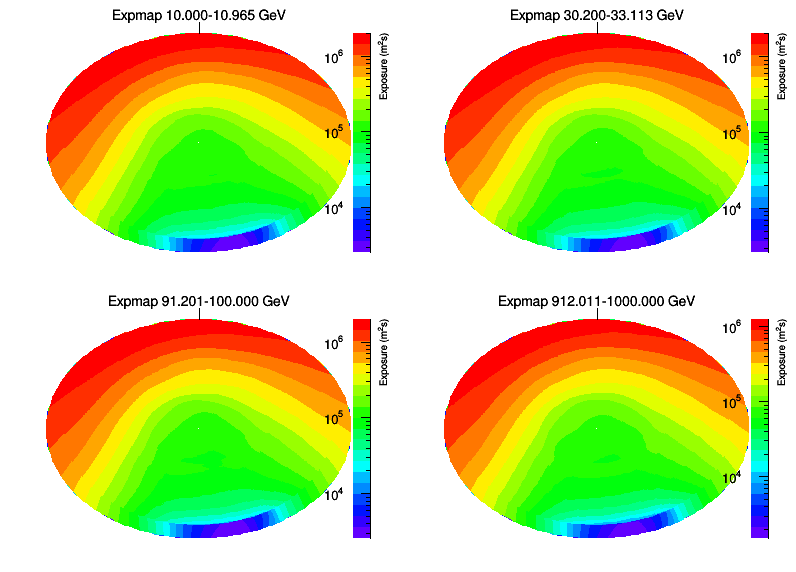
\includegraphics[width=\textwidth]{img/expmapAfterCut}};
    \node [opacity=0.2] (0,0) {\rotatebox{45}{\scalebox{3.0}{\textcolor{red}{preliminary}}}};
    \end{tikzpicture}
    \caption{Exposure map}
\end{figure}

\begin{figure}[h!]
    \begin{tikzpicture}
    \node (0,0) {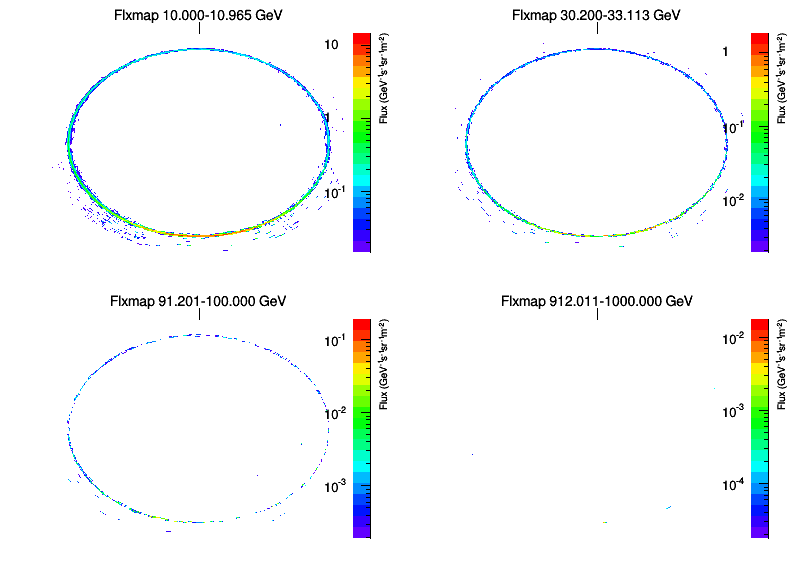
\includegraphics[width=\textwidth]{img/flxmapAfterCut}};
    \node [opacity=0.2] (0,0) {\rotatebox{45}{\scalebox{3.0}{\textcolor{red}{preliminary}}}};
    \end{tikzpicture}
    \caption{Flux map}
\end{figure}
 
\begin{figure}[h!]
    \begin{tikzpicture}
    \node (0,0) {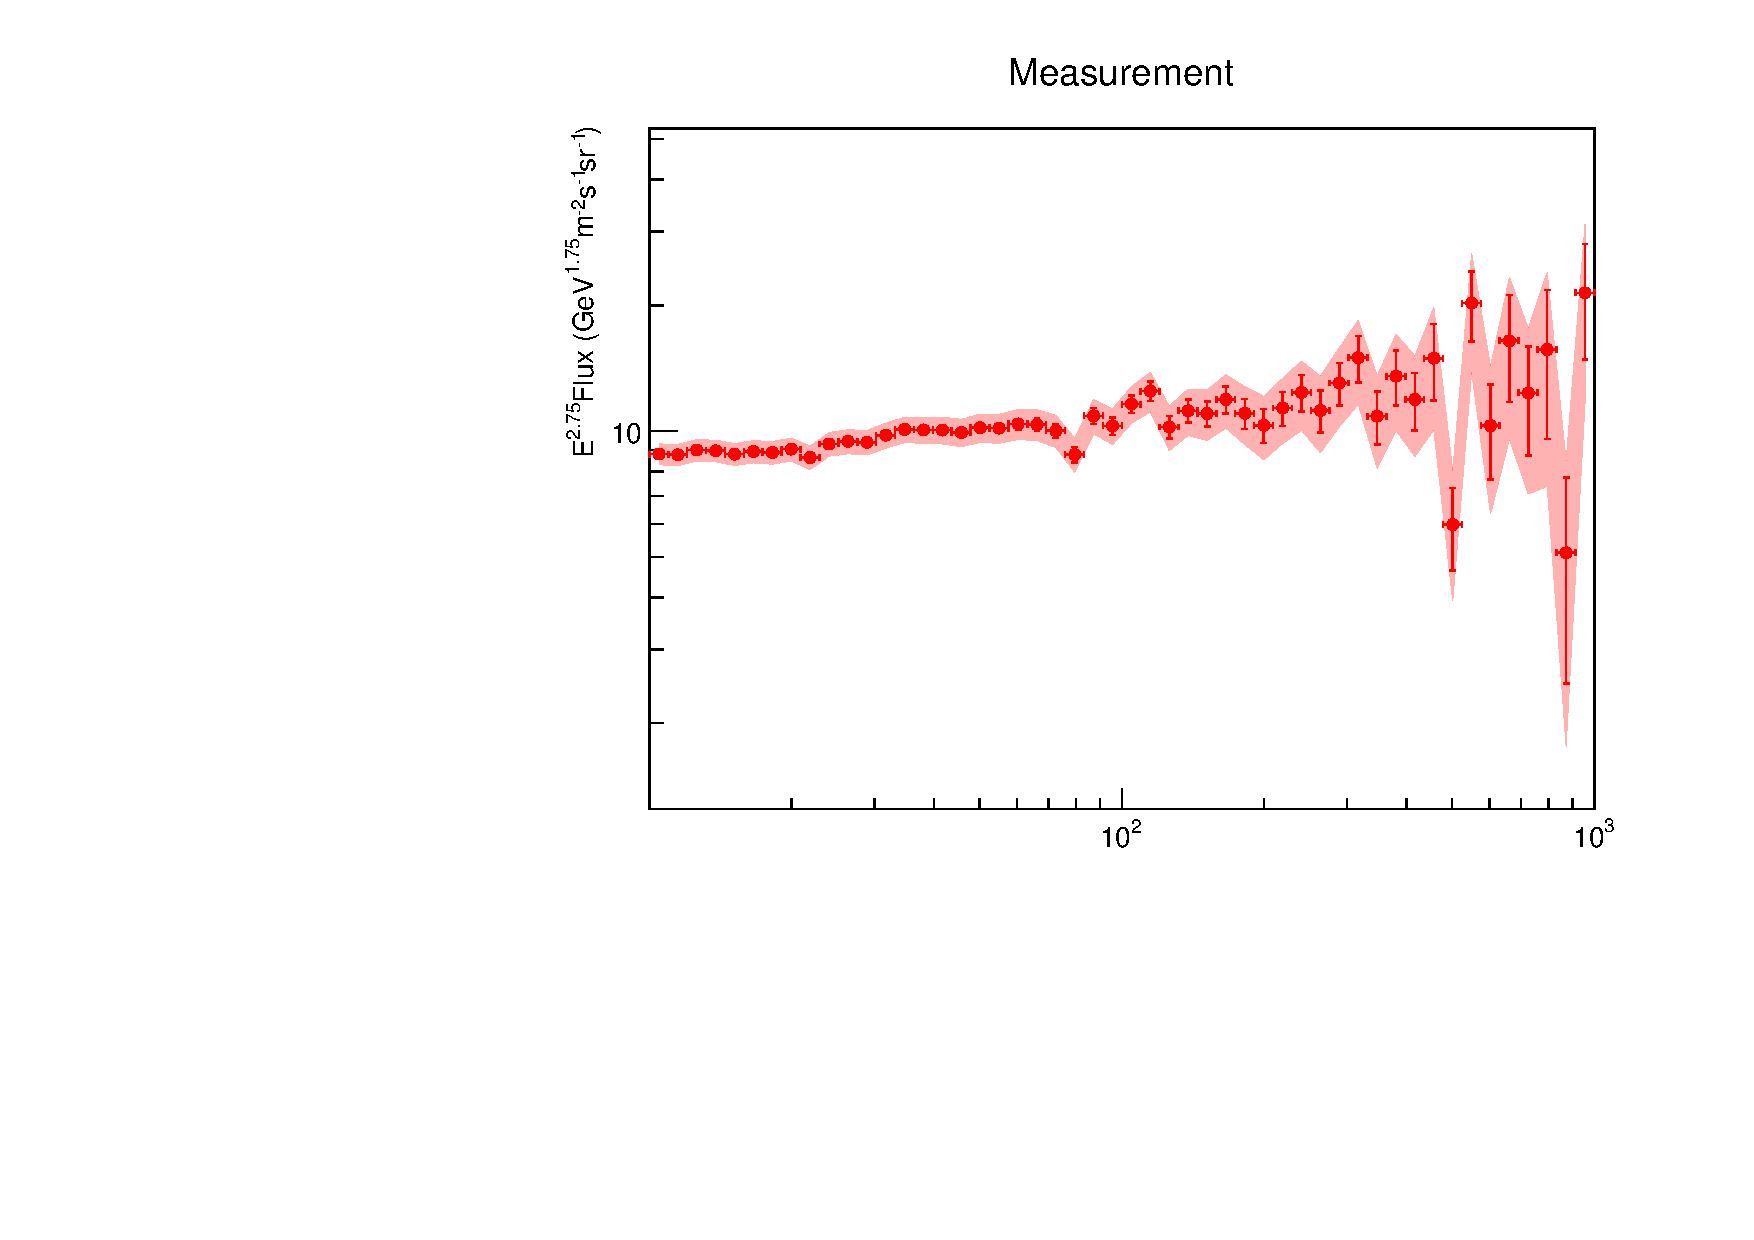
\includegraphics[width=\textwidth]{img/FluxFromExposure}};
    \node [opacity=0.2] (0,0) {\rotatebox{45}{\scalebox{3.0}{\textcolor{red}{preliminary}}}};
    \node [opacity=1.0] at (4.9,-4.7) {E (GeV)};
    \end{tikzpicture}
    \caption{$\gamma$-ray energy spectrum}
\end{figure}


%%%%%%%%%%%%%%%%%%%%%%%%%%%%%%%%%%%%%%%
%%%%%  Power law from measurement   %%%
%%%%%%%%%%%%%%%%%%%%%%%%%%%%%%%%%%%%%%%
\clearpage
\section{Power law from indirect measurement}
The measured parameters of SPL and BPL model has been calculated from optimization process has shown in Table 4.1 and we found that BPL fits better than SPL with a significant level of $3.3\sigma$. 
Note that statistical and total (including systematic error) error computed from Monte Carlo Simulation
The demonstration of $\gamma$-ray from model and measurement also represent in Figure 4.6 as well as Figure 4.7 show a renormalized proton spectrum from this work (indirect measurement) compare with other direct measurement.
% table of SPL & BPl parameters with significant ref from Wilk's theorem
\begin{table}[h!]
    \begin{tabular}{l | c | c | c}
      Best fits & $\gamma_1$ & $\gamma_2$ & $E_{\text{Break}}$ (GeV) \\
      \hline \hline
      Single Power Law (SPL) & 2.68 $\pm$ 0.01(0.03) & - & -  \\
      Broken Power Law (BPL) & 2.84 $\pm$ 0.04(0.06) & 2.64 $\pm$ 0.04(0.17) & 328 $\pm$ 151(267)
    \end{tabular}
    \caption{Optimization results : \\ statistical error and total error has shown in table subsequently}
\end{table}

% gmr spectrum
\begin{figure}[h!]
    \begin{tikzpicture}
    \node (0,0) {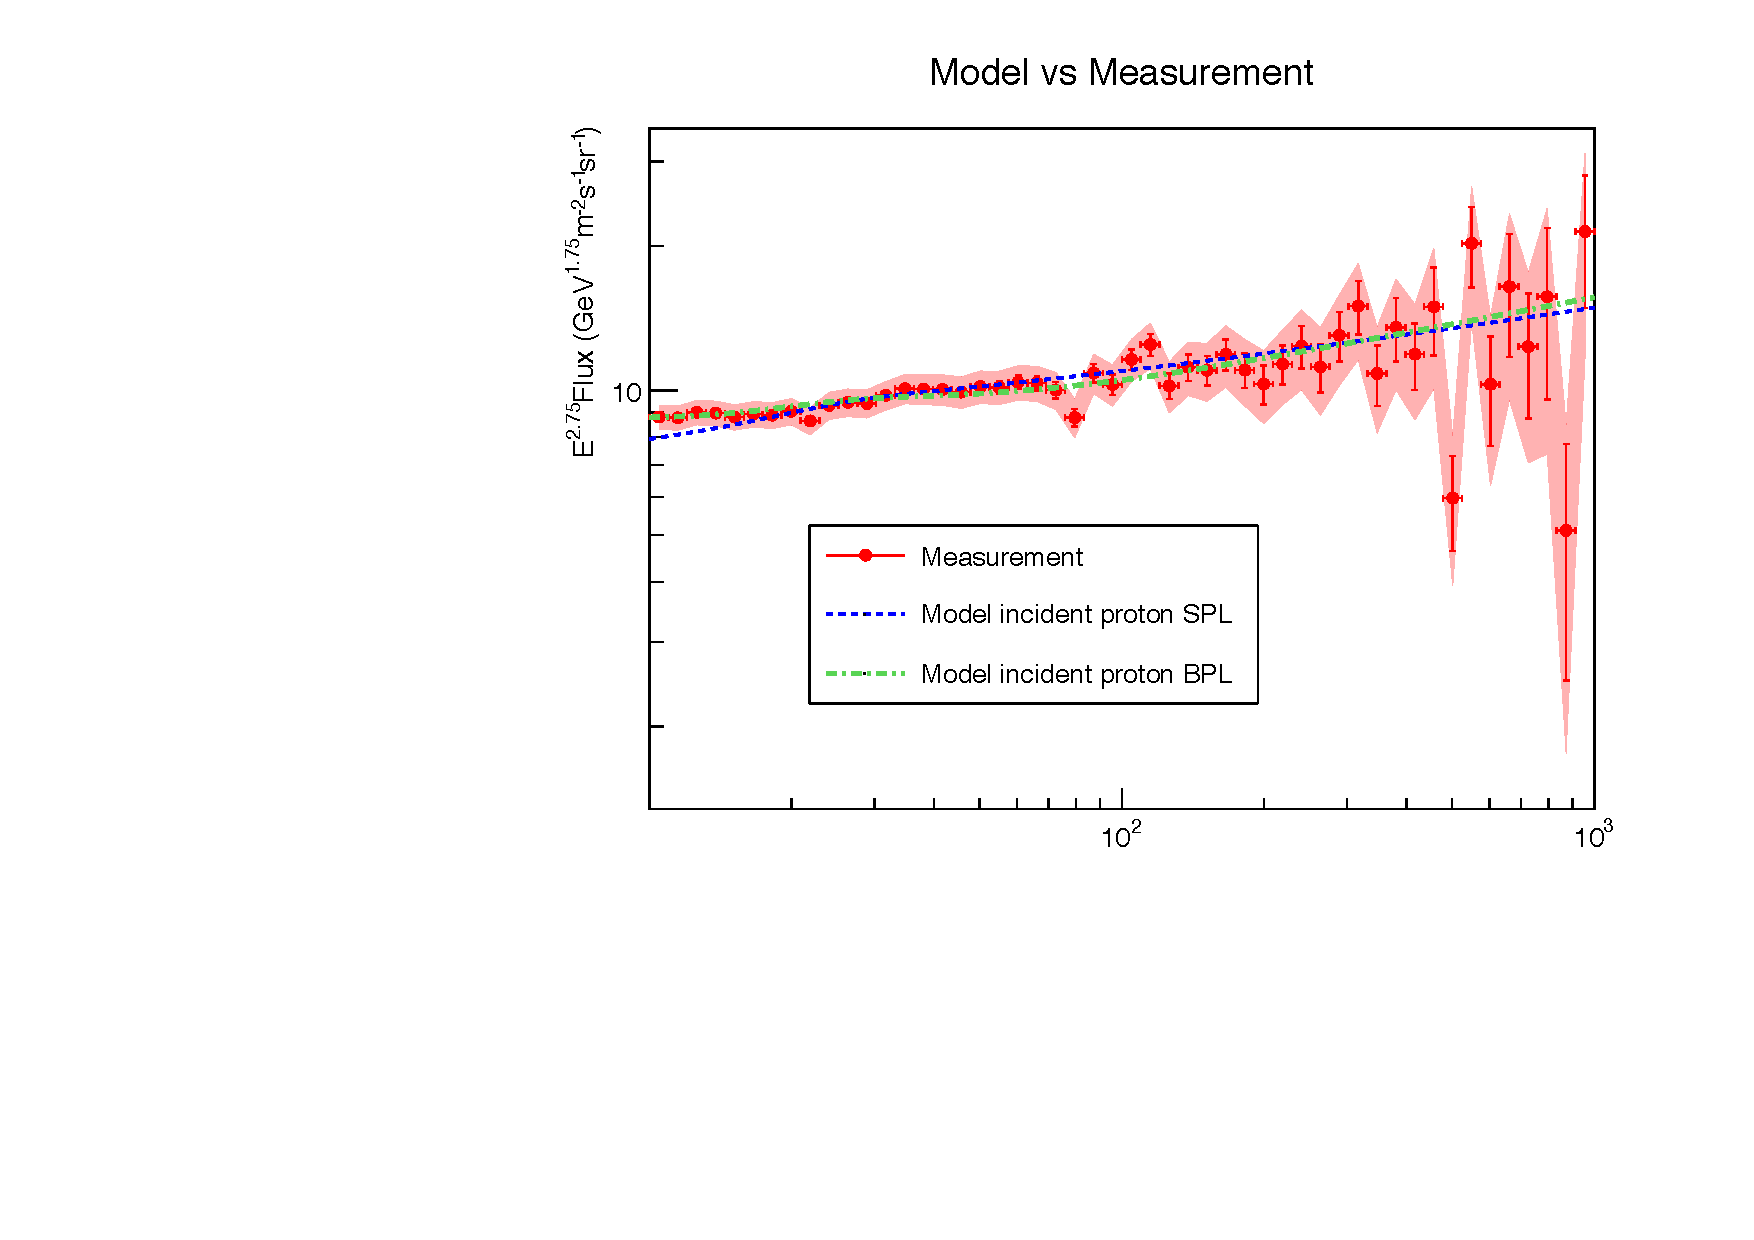
\includegraphics[width=\textwidth]{img/ModelVSMeasurement}};
    \node [opacity=0.2] (0,0) {\rotatebox{45}{\scalebox{3.0}{\textcolor{red}{preliminary}}}};
    \node [opacity=1.0] at (4.9,-4.7) {E (GeV)};
    \end{tikzpicture}
    \caption{$\gamma$-ray spectrum from model and measurement}
\end{figure}

% proton spectrum
\begin{figure}[h!]
    \begin{tikzpicture}
    \node (0,0) {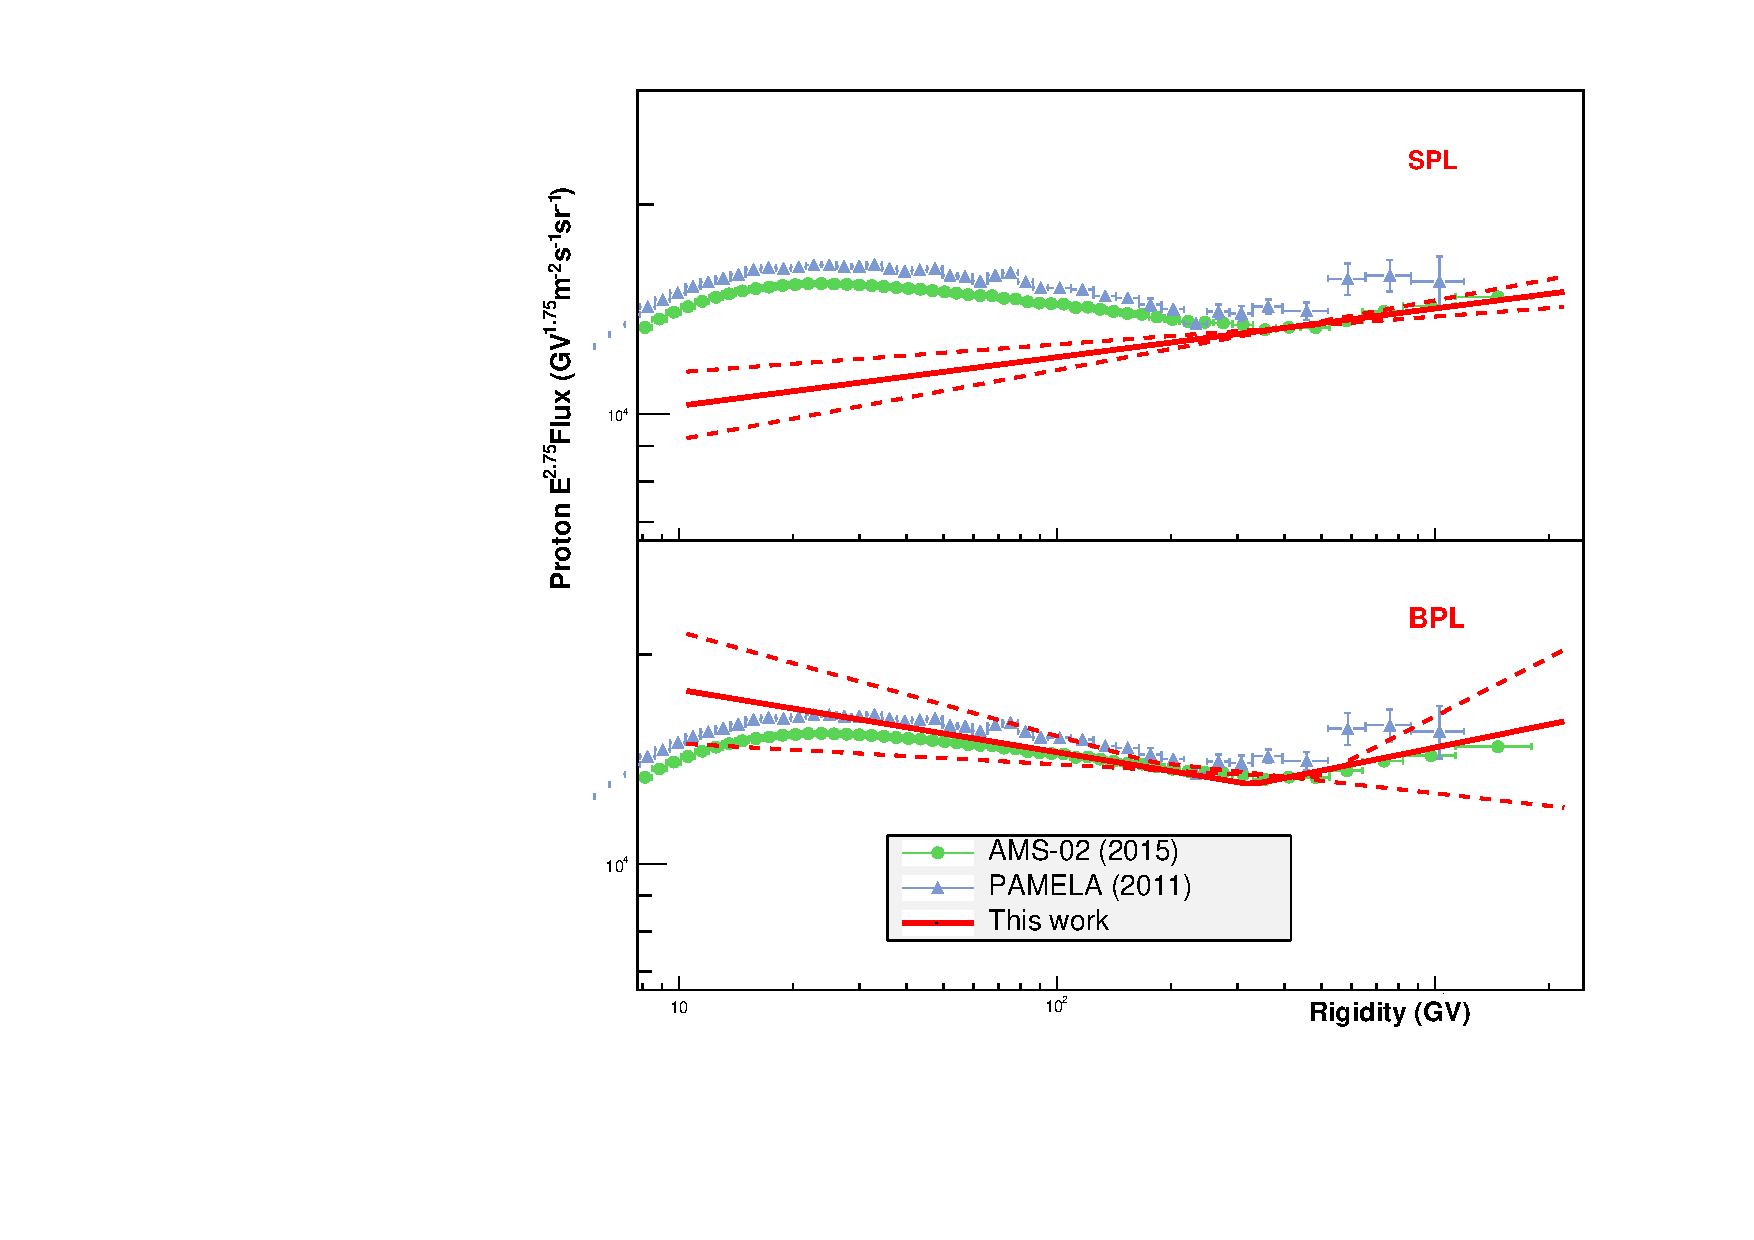
\includegraphics[width=\textwidth]{img/ProtonSpectrumModelMeasurement}};
    \node [opacity=0.2] (0,0) {\rotatebox{45}{\scalebox{3.0}{\textcolor{red}{preliminary}}}};
    \end{tikzpicture}
    \caption{Proton spectrum from model and other direct measurements}
\end{figure}
